\documentclass[a4paper,11pt]{article}
% Various packages
\usepackage{siunitx}
\usepackage[utf8]{inputenc} % æøå
\usepackage[T1]{fontenc} % mere æøå
\usepackage[danish]{babel} % orddeling
\usepackage{verbatim} % så man kan skrive ren tekst
\usepackage{graphicx}
\graphicspath{{assets/}}
\usepackage{a4wide}
\usepackage{url}
\usepackage[left=2cm,top=2cm,bottom=1.5cm,right=2cm]{geometry}
\usepackage{amsmath}
\usepackage{amssymb}
\usepackage{amsthm}
\usepackage{wrapfig}
\usepackage{fixme}
\usepackage{color}
\usepackage{pstricks}
\usepackage{pdfpages} % include pdf
\usepackage{float} % Use [H] in figures
\usepackage{subcaption} % For subfigures
\usepackage{color} % May be necessary if you want to color links
\usepackage{hyperref} % Make references clickable
\usepackage[nameinlink,capitalize]{cleveref} % Make eq:refs be in style (1)
\usepackage[linesnumbered, commentsnumbered, lined, ruled, vlined,
%noend  % Have no ⌊-like symbol to indicate end of scope in pseudocode
]{algorithm2e} % Doc: https://goo.gl/6bC1qZ

% Ændr på navnene der vises når man bruger \autoref{label}
\def\sectionautorefname{Sektion}
\renewcommand{\equationautorefname}{Ligning}
\def\figureautorefname{Figur}
\AtBeginDocument{\renewcommand{\ref}[1]{\autoref{#1}}}

% Sæt \ref{} til at kalde \autoref{}
\AtBeginDocument{\renewcommand{\ref}[1]{\autoref{#1}}}

% Ændr ''*'' i math-felter til \cdot
\DeclareMathSymbol{*}{\mathbin}{symbols}{"01}

% Sæt farver for interne referencer og links
\definecolor{darkblue}{RGB}{25,25,112}
\hypersetup{
	colorlinks=true,    %set true if you want colored links
	linktoc=all,        %set to all if you want both sections and subsections linked
	linkcolor=darkblue, %choose some color if you want links to stand out
	filecolor=blue,     %
	citecolor=black,    %
	urlcolor=cyan,      %
}

% Set indentation to 0:
\setlength\parindent{0pt}

% Keywords relateret til algorithm2e pakken
\newcommand{\True}{\textbf{true}}\newcommand{\False}{\textbf{false}}
\SetStartEndCondition{ }{}{}%
\SetKwProg{Fn}{def}{\string:}{}
\SetKw{KwTo}{to}
\SetKwFor{For}{for}{}{}% 
\SetKwFor{ForEach}{foreach}{}{}% 
\SetKwIF{If}{ElseIf}{Else}{if}{}{elif}{else}{end}% 
\SetKwFor{While}{while}{}{end}\SetKwProg{Fn}{}{}{}
\SetKwInOut{Input}{input}\SetKwInOut{Output}{output}
\setlength{\algomargin}{3em}\DontPrintSemicolon

\newcommand{\longspace}{{\ \ \ \ \ \ \ \ \ \ \ \ \ \ }}
\renewcommand{\P}{{\mathbb P}}
\newcommand{\parfrac}[1]{\frac{\partial}{\partial #1}}
\renewcommand{\num}{{\textrm{num} }}
\newcommand{\size}{{\textrm{size} }}
\newcommand{\ift}{{\textrm{if } }}

% Dynamiske (), <>, ceil, floor
\newcommand{\p}[1]{\left( #1 \right)}
\newcommand{\pbig}[1]{\big( #1 \big)}
\newcommand{\pBig}[1]{\Big( #1 \Big)}
\newcommand{\pbigg}[1]{\bigg( #1 \bigg)}
\newcommand{\larr}[1]{\left< #1 \right>}
\newcommand{\ceil}[1]{\left\lceil #1 \right\rceil}
\newcommand{\floor}[1]{\left\lfloor #1 \right\rfloor}


% Squiggly arrows
\DeclareFontFamily{U} {MnSymbolC}{}

\DeclareFontShape{U}{MnSymbolC}{m}{n}{
	<-6> MnSymbolC5
	<6-7> MnSymbolC6
	<7-8> MnSymbolC7
	<8-9> MnSymbolC8
	<9-10> MnSymbolC9
	<10-12> MnSymbolC10
	<12-> MnSymbolC12}{}
\DeclareFontShape{U}{MnSymbolC}{b}{n}{
	<-6> MnSymbolC-Bold5
	<6-7> MnSymbolC-Bold6
	<7-8> MnSymbolC-Bold7
	<8-9> MnSymbolC-Bold8
	<9-10> MnSymbolC-Bold9
	<10-12> MnSymbolC-Bold10
	<12-> MnSymbolC-Bold12}{}

\DeclareSymbolFont{MnSyC} {U} {MnSymbolC}{m}{n}

\DeclareMathSymbol{\MNrhd}{\mathbin}{MnSyC}{76}
\DeclareMathSymbol{\MNlhd}{\mathbin}{MnSyC}{78}
% =============================================
\DeclareFontFamily{U} {MnSymbolD}{}

\DeclareFontShape{U}{MnSymbolD}{m}{n}{
	<-6> MnSymbolD5
	<6-7> MnSymbolD6
	<7-8> MnSymbolD7
	<8-9> MnSymbolD8
	<9-10> MnSymbolD9
	<10-12> MnSymbolD10
	<12-> MnSymbolD12}{}
\DeclareFontShape{U}{MnSymbolD}{b}{n}{
	<-6> MnSymbolD-Bold5
	<6-7> MnSymbolD-Bold6
	<7-8> MnSymbolD-Bold7
	<8-9> MnSymbolD-Bold8
	<9-10> MnSymbolD-Bold9
	<10-12> MnSymbolD-Bold10
	<12-> MnSymbolD-Bold12}{}

\DeclareSymbolFont{MnSyD} {U} {MnSymbolD}{m}{n}
\DeclareMathSymbol{\MNsim}{\mathbin}{MnSyD}{2}

% =============================================

\usepackage{amssymb,amsmath,stackengine}
\stackMath
\newcommand\rsquigarrow[1]{%
	\mathbin{\stackon[2pt]{\rightsquigarrow}{\scriptscriptstyle #1 }}
}

\author{Søren Mulvad, rbn601}

\title{Eksamensdisposition - Fibonacci Heaps}

\begin{document}
\maketitle

% Desuden skal hver studerende i gruppen udarbejde en individuel disposition for emnet "Binære søgetræer", som er et af emnerne til eksamen. En disposition skal bestå af de vigtigste punkter, du vil komme ind på til eksamen.
% Tænk på dispositionen som noget, du kan have med dig til eksamen, og som kan hjælpe dig med at huske, hvad du overordnet vil gennemgå til emnet "Binære søgetræer".
% Dispositionen skal ikke indeholde detaljerede beviser og lignende, men de mere overordnede delemner. Sørg for at gøre den kortfattet - f.eks. 5-10 punkter med stikord/-sætninger.


\begin{itemize}
\item \textbf{Motivation}


\item \textbf{Struktur}
\begin{itemize}
	\item Egenskaber
	\item Pointers/attributter
	\item Operationer
\end{itemize}


\item \textbf{Håndkørsel af \texttt{Extract-Min}}
\begin{figure}[H]
	\begin{center}
		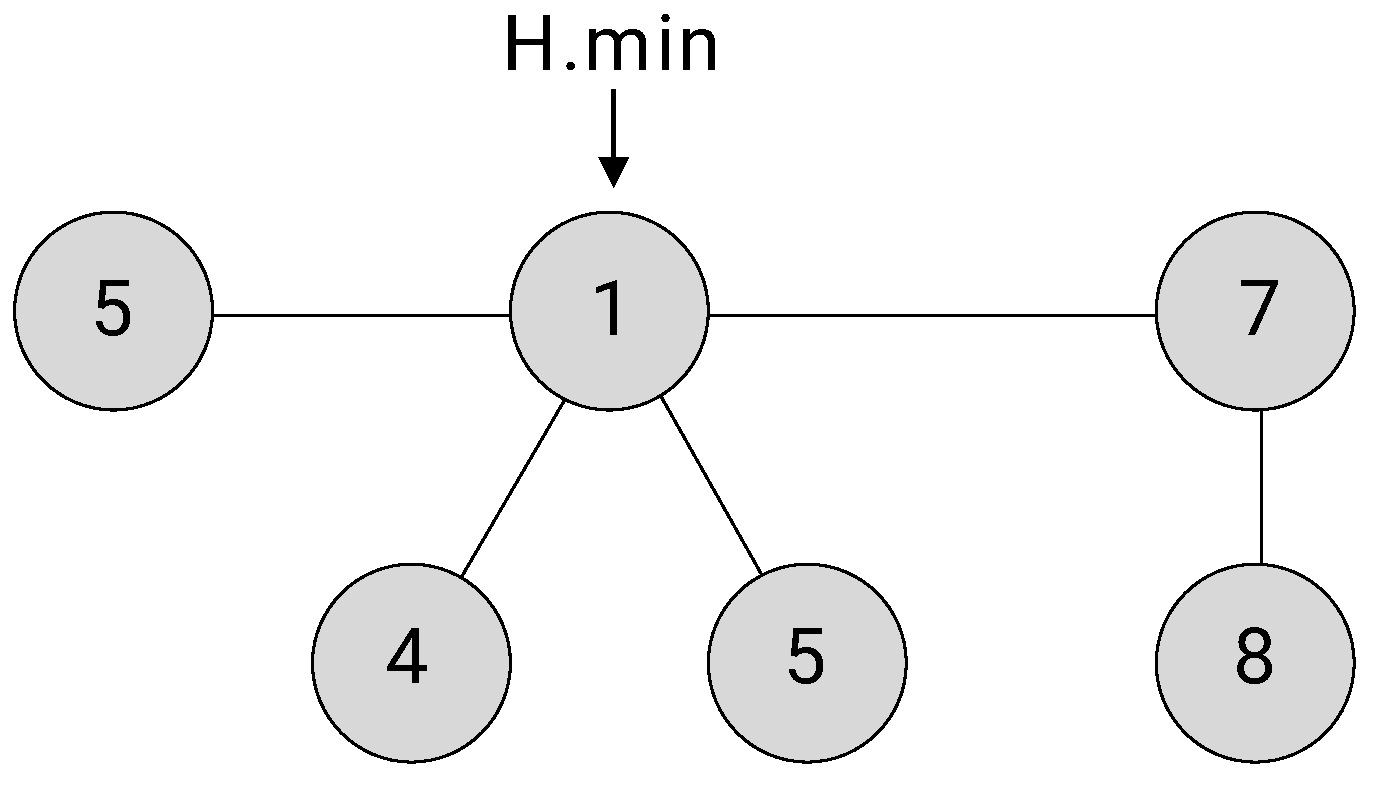
\includegraphics[width=0.4\textwidth]{extract-min-simple.pdf}
	\end{center}
\end{figure}

\item \textbf{Potentialefunktionen}
%\begin{itemize}
%	\item Definér potentialefunktion: $\Phi(H) \ = \ \underbrace{t(H)}_{\text{\makebox[0pt]{Antal rod-knuder}}} \ + \ 2   \overbrace{m(H)}^{\text{\makebox[0pt]{Antal markerede knuder}}}$.
%	\item Antag $D(n) = O(\lg n)$.
%\end{itemize}

\item \textbf{Amortiseret køretid for \texttt{Extract-Min}}

\item \textbf{Håndkørsel af \texttt{Decrease-Key}}
\item \textbf{Amortiseret køretid for \texttt{Decrease-Key}}

\end{itemize}

%%%%%%%%%%%%%%%%%%%%%%%%%%%%%%%%%%%%%%%%%%%%%%%%%%%%%%%%%%%
%%%%%%%%%%%%%%%%%%%%%%%%%%%%%%%%%%%%%%%%%%%%%%%%%%%%%%%%%%%
%%%%%%%%%%%%%%%%%%%%%%%%%%%%%%%%%%%%%%%%%%%%%%%%%%%%%%%%%%%
\newpage
%%%%%%%%%%%%%%%%%%%%%%%%%%%%%%%%%%%%%%%%%%%%%%%%%%%%%%%%%%%
%%%%%%%%%%%%%%%%%%%%%%%%%%%%%%%%%%%%%%%%%%%%%%%%%%%%%%%%%%%
%%%%%%%%%%%%%%%%%%%%%%%%%%%%%%%%%%%%%%%%%%%%%%%%%%%%%%%%%%%
\section{Fibonacci Heaps}



\begin{itemize}
\item \textbf{Motivation}
\begin{itemize}
	\item God amortiseret køretid, mange af operationerne er i konstant tid.
	\item Gør den velegnet til applikationer som benytter den mange gange. Særligt når \texttt{Extract-Min} og \texttt{Delete} bliver kaldt få gange relativt set.
	\item Bl.a. Dijkstra's algoritme og Prim's algoritme (Minimum Spanning Trees) gør brug af Fibonacci Heaps.
	\item Ligesom vi her vil tale om en Min-Heap kunne man ligeledes lave en Max-Heap.
\end{itemize}



\item \textbf{Struktur}

\begin{itemize}
	\item Min-heap-egenskab: Key'en for en knude er altid $\geq$ key'en for dens forælder. En heap $H$ har pointeren $H.min$ til minimumsknuden ved roden af træet.
	\item Knuden $x$ har pointerne/attributerne
	\begin{itemize}
		\item $x.p$ - Forælder-knude
		\item $x.child$ - En vilkårlig af børnene
		\item $x.left$ og $x.right$
		\item $x.mark$ - Sandhedsværdi som markerer om knuden har mistet ét barn siden den sidst blev gjort til et barn af en anden knude. Nye knuder er umarkerede, og bliver derudover umarkerede hver gang de bliver gjort til barnet af en anden knude.
		\item $x.degree$ - Antallet af børn i barnelisten (f.eks. for knuden $x$ med $x.key = 3$ i figuren nedenfor er $x.degree = 3$).
	\end{itemize}
	
	\item Når en Fibonacci Heap $H$ er tom er $H.min = NIL$.
	\item Vi bruger en cirkulær doubly linked lists til at forbinde rodknuderne og børnelisterne for en bestemt knude (se nedenfor for illustration):
	
	\begin{figure}[H]
		\begin{center}
			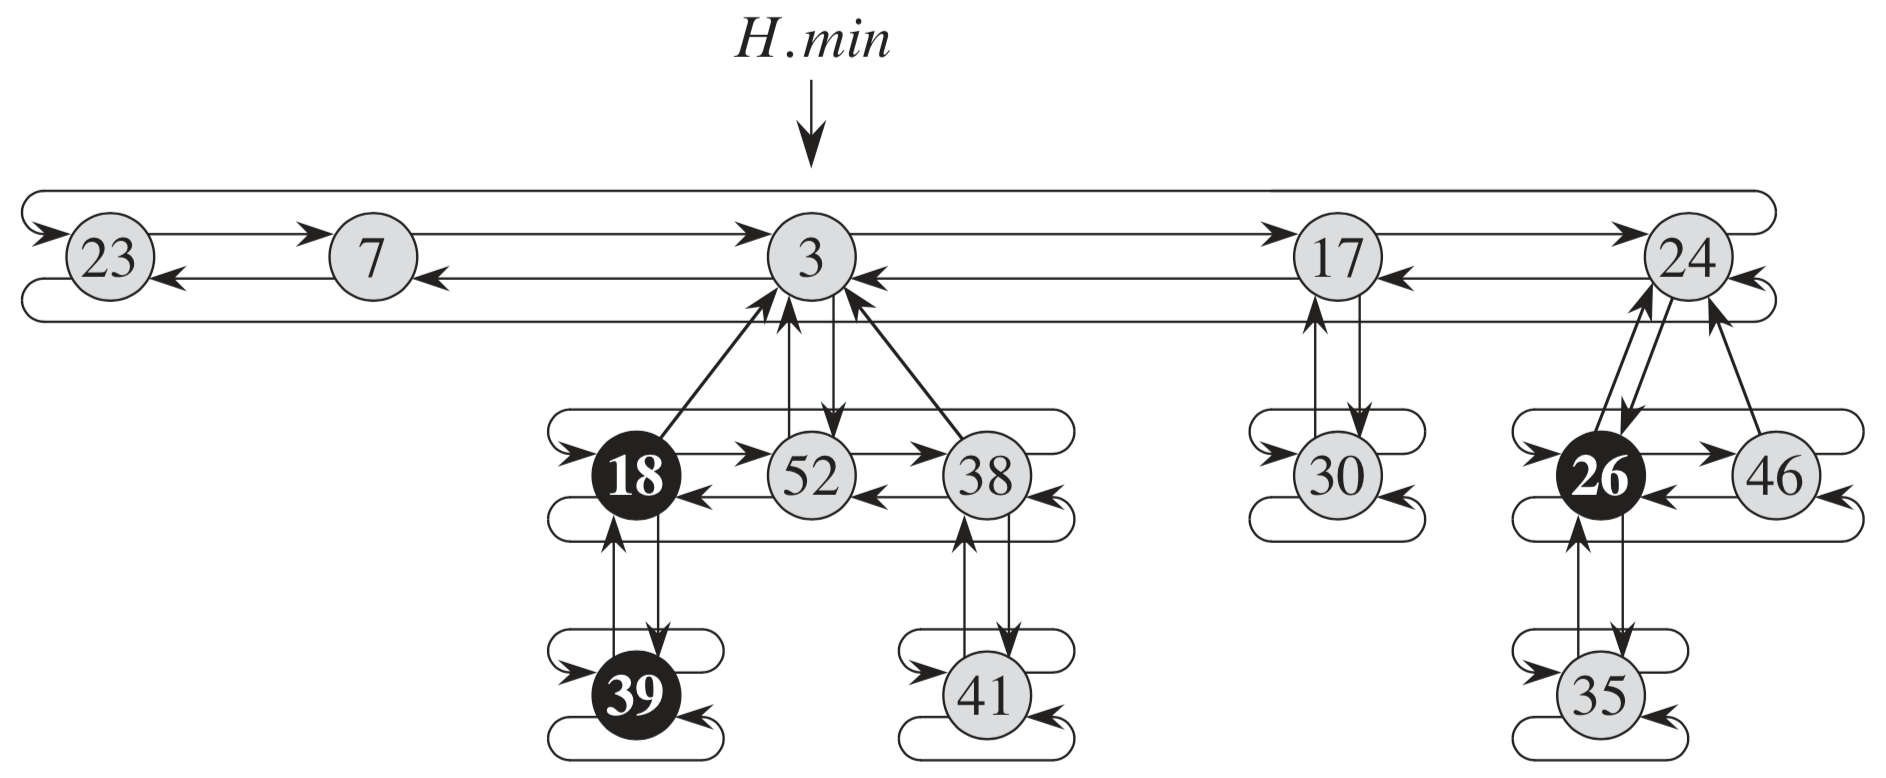
\includegraphics[width=0.7\textwidth]{linked.png}
		\end{center}
	\end{figure}
	
	
	\item Operationernes amortiserede køretid og argumenter ($H =$ heap, $x =$ knude og $k =$ ny key):
	\begin{table}[H]
		\centering
		\begin{tabular}{lc}
			\textbf{Operation}               & \multicolumn{1}{l}{\textbf{Amortiseret køretid}} \\ \hline
			\texttt{Make-Heap}$()$           & $\Theta(1)$                                      \\
			\texttt{Insert}$(H, x)$          & $\Theta(1)$                                      \\
			\texttt{Minimum}$(H)$            & $\Theta(1)$                                      \\
			\texttt{Union}$(H_1, H_2)$       & $\Theta(1)$                                      \\
			\texttt{Decrease-Key}$(H, x, k)$ & $\Theta(1)$                                      \\
			\texttt{Extract-Min}$(H)$        & $\Theta(\lg n)$                                  \\
			\texttt{Delete}$(H, x)$          & $\Theta(\lg n)$
		\end{tabular}
	\end{table}
	\item Det tager lang tid at søge efter et element, så i ovenstående køretider antager vi at vi allerede har en pointer direkte til den knuden $x$ vi gerne vil udføre en operation ved.
\end{itemize}

\item \textbf{Håndkørsel af \texttt{Extract-Min}}\\
Her er hoben før operationen og hoben efter tegnet. \texttt{Extract-Min} er det hvor vi laver et array $A[0..D(n)]$ og ser på degree af hver knude i roden.
\begin{figure}[H]
	\begin{center}
		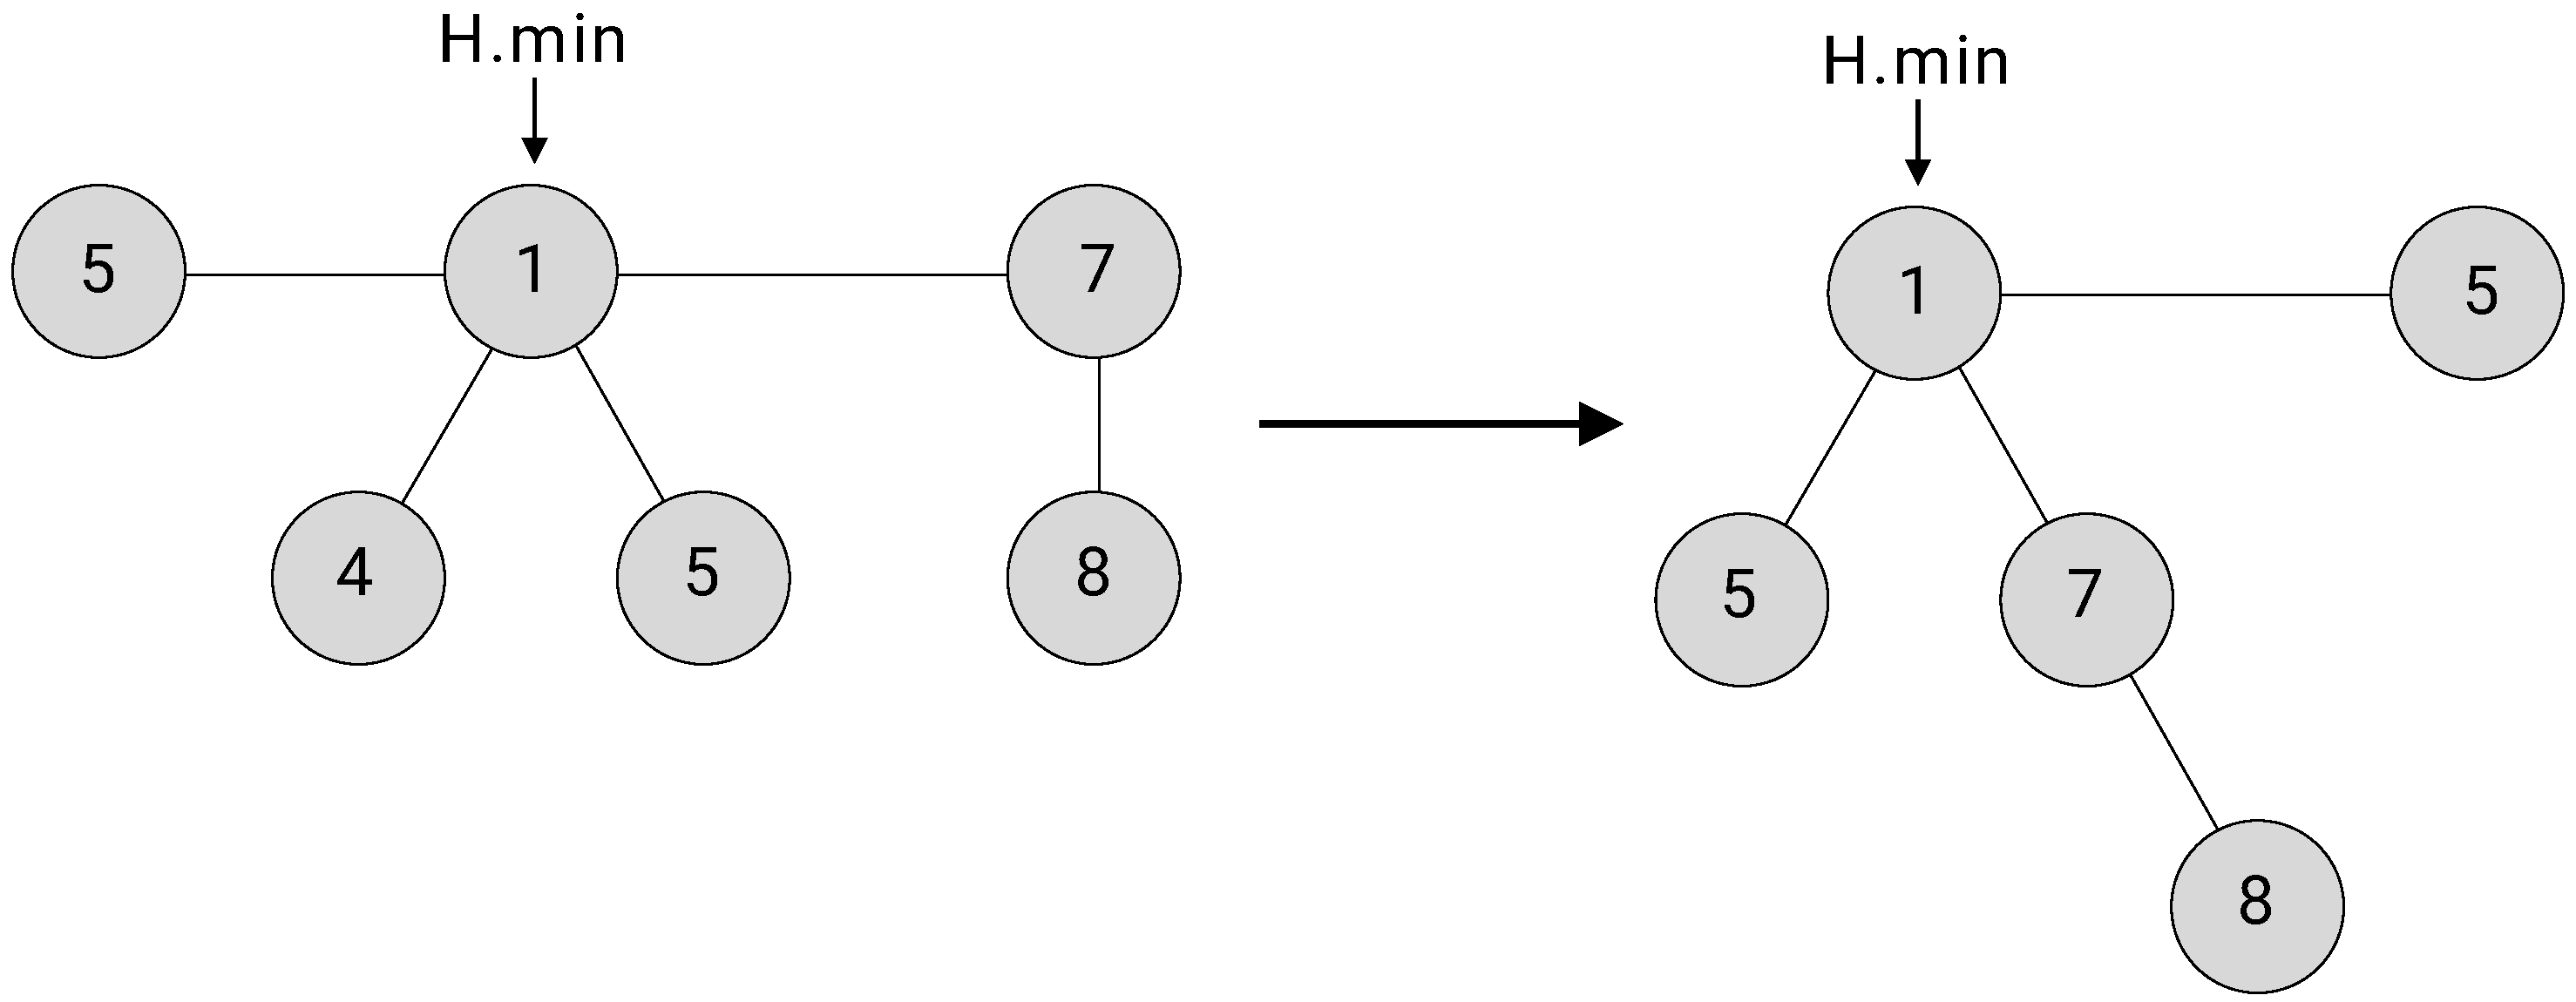
\includegraphics[width=0.9\textwidth]{extract-min.pdf}
	\end{center}
\end{figure}


\item \textbf{Håndkørsel af \texttt{Decrease-Key}}\\
Tegn en ekstra knude under 7 på det træ du kom frem til før. Fjern knuderne med key 10 og key 8. Træet før vi begynder, efter første decrease og efter andet decrease vil se således ud:
\begin{figure}[H]
	\begin{center}
		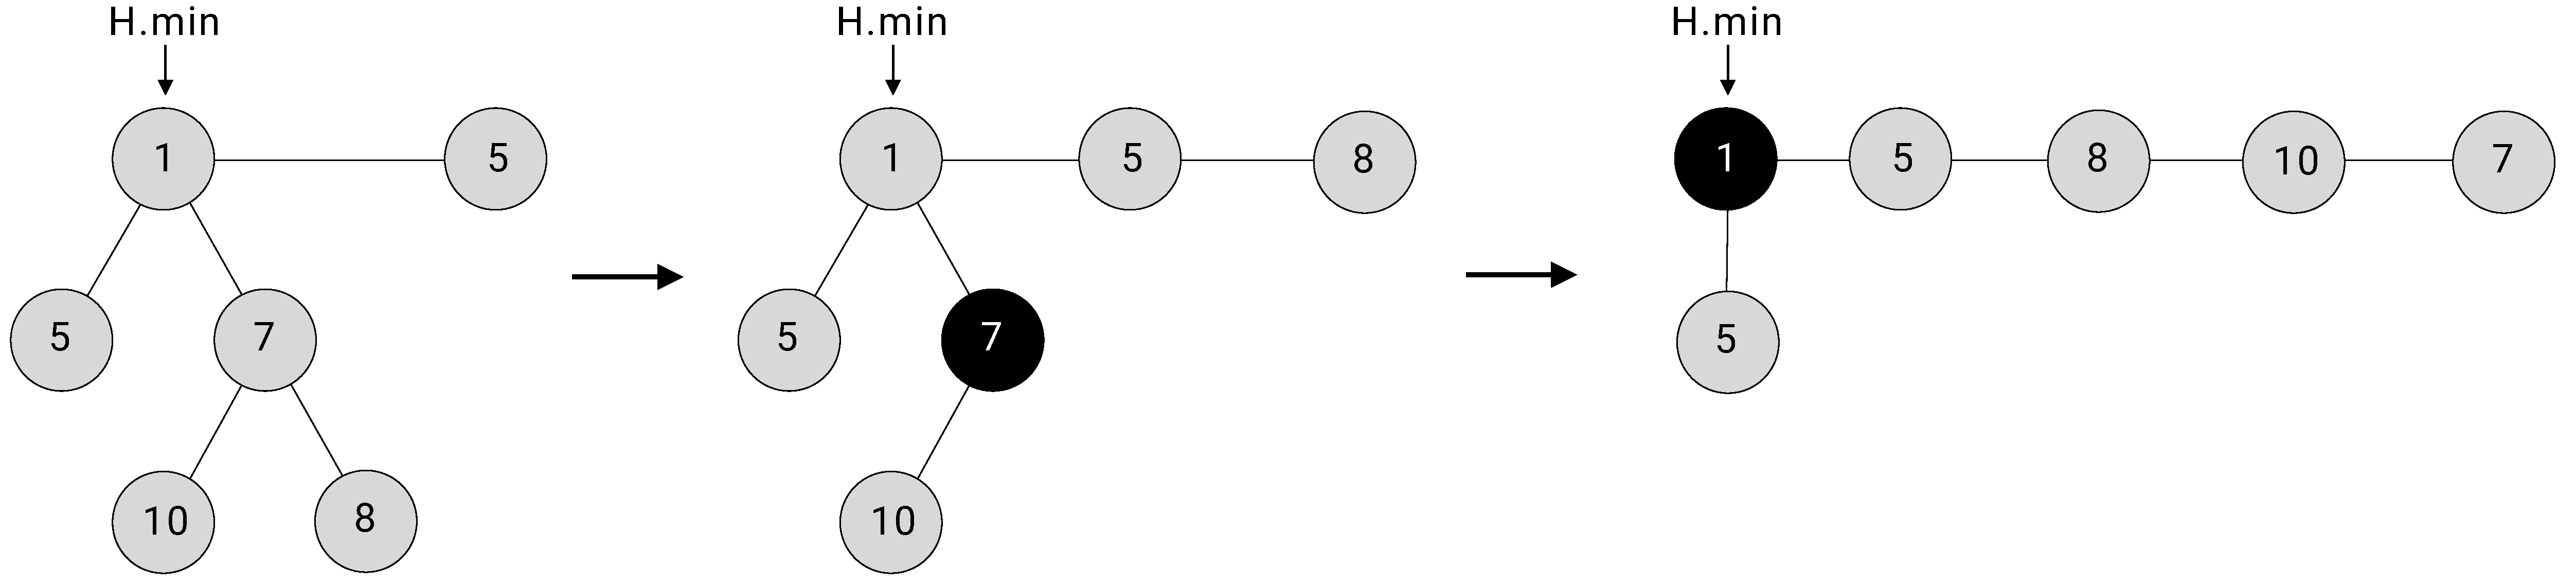
\includegraphics[width=1\textwidth]{decrease-key.pdf}
	\end{center}
\end{figure}
% Lynhurtig forklaring: Man nedsætter værdien for ens knude $x$ og flytter den op i roden. Hvis den forælder ikke er markeret så markerer man nu den, men mere sker ikke. Hvis forælderen er markeret i forvejen, så flyttes den også op i roden (og dens forælder reagerer ligeledes på den har mistet sit barn osv.)


\item \textbf{Potentialefunktion}
\begin{itemize}
	\item Definer potentialefunktionen:
	$$
	\Phi(H) \ = \ \underbrace{t(H)}_{\text{\makebox[0pt]{Antal rod-knuder}}} \ + \ 2   \overbrace{m(H)}^{\text{\makebox[0pt]{Antal markerede knuder}}}
	$$
	
	\item Gyldighed: Vi ser at den er gyldig, da idet der er ingen knuder i vors Fib-Heap vil den være 0. Ellers kan der kun være et positivt antal knuder og/eller markerede knuder, og derfor vil den ellers altid være positiv.
	
	\item Den amortiserede cost af enhver operation er dens faktiske cost plus ændringen i potentialet. Den totale amortiserede cost af $n$ operationer er: \textit{(Vi ved dette fra kapitel 17, uddyb ikke)}
	$$
	\sum_{i=1}^n \hat c_i = \p{ \sum_{i=1}^n c_i } + \Phi(D_n) - \Phi(D_0)
	$$
	
	\item Antag øvre grænse $D(n) = O(\lg n)$ for den maksimale degree på enhver knude i en $n$-knude stor Fib-Heap. \textit{(Kursorisk, skal ikke bevises)}
\end{itemize}

\newpage
\item \textbf{Bevis for amortiseret køretid for \texttt{Extract-Min} (s. 517 bund - 518)}
\begin{itemize}
		\item[Faktisk cost:] $O(D(n))$ fra først maksimalt at flytte $D(n)$ børn op i roden og for at initialisere vores $D(n)$ lange degree-liste $A$ samt at finde $H.min$ til sidst.
		
		Derudover får vi i værste fald at antallet af rod-knuder lige efter at have \texttt{Consolidate}'d er $D(n) + t(H) - 1$ hvor:
		$$
		\underbrace{D(n)}_{\text{\makebox[50pt]{Børnene fra den udtrakte knude}}} + \overbrace{t(H)}^{\text{\makebox[50pt]{De originale rodknuder}}} \underbrace{- 1}_{\text{\makebox[50pt]{Det udtrakte element}}}
		$$
		
		Vi ved, at vi hver eneste gang i loopet enten rykker én frem eller linker to knuder sammen, og derfor er det totale arbejde i værste fald følgende, hvor vi antager uligheden:
		$$
		O \pBig{ D(n) + t(H) } \leq D(n) + t(H)
		$$
		
		
		\item[Potentiale:] Potentialet før er $t(H) + 2m(H)$\\
		Potentialet efter er $(D(n) + 1) + 2m(H)$ (siden højest $D(n) + 1$ rødder er tilbage da det er længden af vores array $A$ og ingen knuder bliver markeret).
		
		\item[Udregning:]
		\begin{align}
		\hat c_i &= c_i + \Phi(H') - \Phi(H)\\
		    &= D(n) + t(H) + \pBig{(D(n) + 1) + 2m(H)} - \pBig{ t(H) + 2m(H) } \label{eq:reduce} \\
		    &= 2D(n) + 1 \label{eq:dominate} \\
		    &= O(D(n)) \nonumber \\
		    &= O(\lg n) \nonumber
		\end{align}		
		
		\item[Intuition:] Vores cost af at udføre hver eneste link af to knuder bliver betalt for af reduktionen i potentialet der sker når et link reducerer antallet af knuder i træet med 1.
\end{itemize}



\item \textbf{Bevis for amortiseret køretid for \texttt{Decrease-Key} (s. 520-522)}
\begin{itemize}
	\item[Faktisk cost:] Selve det at formindske vores key tager konstant tid. Herefter kan der være $c$ kald hvor forælderknuderne går fra sand til falsk så de skal flyttes op i roden, som hver for sig tager konstant tid, hvorved vi får en køretid på $c$.
	
	\item[Potentiale:] For alle $c$ rekursive kald pånær det sidste fjerner vi markeringen for forælderknude og flytter vores nuværende knude op i roden. Altså vil der efter udførslen være følgende antal træer:
	$$
	t(H') = t(H) + c
	$$
	
	Derudover vil der højst være følgende antal markerede knuder, da $c-1$ træer blev umarkeret i processen, mens den allersidste muligvis blev markeret:
	$$
	m(H') = m(H) - c + 2
	$$
	
	\item[Udregning:] Ændringen i potentiale vil højst være:
	\begin{align*}
	\Phi(H') - \Phi(H)
	&= \pBig{ (t(H) + c) + 2(m(H) - c + 2) } - \pBig{ t(H) + 2m(H) }\\
	&= \pBig{ (t(H) + c) + 2m(H) - 2c + 4 } - \pBig{ t(H) + 2m(H) }\\
	&= 4 - c
	\end{align*}
	
	Herved fås den amortiserede køretid til at være:
	$$
	\hat c_i = c + (4 - c) = O(1)
	$$
	
\end{itemize}
\end{itemize}
\end{document}